\documentclass{pracamgr}  
\usepackage{lmodern} 
\usepackage[polish]{babel} 
\selectlanguage{polish} 
\usepackage{fontspec}
\usepackage{minted}
\usepackage{listings}
% package for hyperinks
\usepackage{hyperref}
\hypersetup{
    colorlinks,
    citecolor=black,
    filecolor=black,
    linkcolor=black,
    urlcolor=black
}
\usepackage{graphicx}  
\usepackage{makeidx}\makeindex
 
%Jesli uzywasz kodowania polskich znakow ISO-8859-2 nastepna linia powinna byc odkomentowana
%Jesli uzywasz kodowania polskich znakow CP-1250 to ta linia powinna byc 
%odkomentowana
%\usepackage[cp1250]{inputenc}

% Dane magistranta:

\author{Konrad Lisiecki}
\nralbumu{48211}
\title{Modele zmienności stochastycznej} 
\kierunek{Finanse i rachunkowość}
\instytut{Ekonometrii}
\opiekun{dra hab. Łukasza Delonga} 
\date{Warszawa 2015}   

% Tu jest dobre miejsce na Twoje własne makra i~środowiska:
\newtheorem{defi}{Definicja}[section]

% koniec definicji 

%\makeindex[intoc] 
 


%===========================================================================
%             Bibliogrphy
%=========================================================================== 
\usepackage[style=numeric,sorting=ydnt,defernumbers=true, backend=bibtex]{biblatex}
\addbibresource{biblio.bib}
 

%===========================================================================
%                           Begin of document 
%===========================================================================


\begin{document}
\maketitle
\nocite{book-full} 

%===========================================================================
%                               Introduction
%===========================================================================
\chapter*{Streszczenie} 

\begin{quote}
We developed what is known a stochastic volatility model. This is a model where the volatility as well as the underlying asset price moves around in an unpredictable way.
\raggedleft\slshape John Hull \index{Hull John}
\end{quote}



%===========================================================================
%                               Table of contents
%===========================================================================
\tableofcontents
 

\addcontentsline{toc}{chapter}{Introduction} \markboth{INTRODUCTION}{}


%===========================================================================
%                               Wprowadzenie
%===========================================================================
\chapter{Wprowadzenie}\label{r:pojecia}
\begin{quote}

Never think that lack of variability is stability. Don't confuse lack of volatility with stability, ever.
 
\raggedleft\slshape Nassim Nicholas Taleb \index{Taleb Nassim Nicholas}
\end{quote}
 


adsafdsdfs
 
\section{Definicje}
dsfdsf

\begin{defi}\label{aa}
fsdf
\end{defi}

\begin{defi}\label{aaa}
sdfsdf
\end{defi}




%===========================================================================
%                               Model Hestona
%===========================================================================
\chapter{Model Hestona}
\begin{quote}
  Suppose we use the standard deviation ... of possible future returns on
  a stock ... as a measure of its volatility. Is it reasonable to take
  that volatility as a constant over time? I think not.

\raggedleft\slshape Fisher Black \index{Fisher, Black}
\end{quote}

Obecnie jednym z najpopularniejszych narzędzi do wyceny opcji jest model Blacka-Scholsa. Ceniony jest on ze względu na prostotę oraz wygodę użycia, kosztem jednak wielu upraszczających założeń. Jednym z najważniejszych jest założenia o stałej zmienności instrumentu bazowego, co w znaczącym stopniu ogranicza precyzje oszacowań. Jednym z pomysłów na obejście tego problemu jest uzmiennienie tej stałej, czyli pozwolanie, aby dla dowolnego czasu, parametr ten przyjmował różną wartość. Można to zrobić np. poprzez pozwolenie, aby nie tylko proces ceny akcji był procesem stochastycznym, ale także aby sama zmienność była niedetrministyczna, tzn. aby była również definiowana przy użyciu procesu stochastycznego. Takie też podejście zostało wykorzystane przy budowie modelu Hestona. \cite{greenwade93}

\section{Model Blacka-Scholesa}

Jak zostalo wspomniene we wstepie podstawowym modelem matematycznym na wycenę opcji jest model Blacka-Scholesa. Najczęściej definiuje się go w następującej postaci:
\begin{equation}
dS_t  = \mu S_t dt + \sigma S_t dW^S_t
\end{equation}

We wzorze tym $S_t$ przedstawia cenę instrumentu bazowego w momencie $t$, stała $\mu$ oznacza dryf, stała $\sigma$ oznacza zmienność, natomiast $dW^S_t$ jest standardowym procesem Wienera (procesem błądzenia losowego).

Ze względu na swoją prostotę, model ten jest podstawową metodą do wyceny opcji, jednak wspomniana prostota niesie za sobą szereg ograniczeń. Jednym z takich ograniczeń jest założenie o stałej wartości zmienności w czasie. Jak bardzo to założenie potrafi być niezgodne z rzeczywistością pokazał chociażby ostatni kryzys finansowy, podczas którego zmiennośc instrumentów finansowych była o wiele większa niż w poprzednich latach. Dlatego też naturalnym uogónieniem modelu Blacka-Scholesa wydaje się być wprowadzenie zmienności, która nie jest stała. Taką zmianę wprowadza model Hestona. 

\section{Model Hestona}

Na początek załóżmy, że cena aktywa bazowego w momemcie $t$ spełnia następujący proces dyfuzji:
\begin{equation}
dS(t)= \mu S dt + \sqrt{v(t)} S d z_1 (t),
\end{equation}
gdzie $z_1(t)$  jest standardowym procesem Wienera. 

Jeżeli natomiast zmienność jest procesem Ornsteina-Uhlenbecka:

\begin{equation}
d \sqrt{v(t)} = - \beta \sqrt{v(t)} dt + \delta d z_2 (t)
\end{equation}

wtedy na podstawie lematu Ito można wykazać, że wariancja $v(t)$ ma nastepującą postać:
\begin{equation}
dv(t)= \kappa  [\theta -v(t)]dt+2\delta \sqrt{v(t)} d z_2 (t)
\end{equation}
gdzie proces $z_2(t)$ ma korelację z procesem $z_1(t)$ równą $\rho$.

Gdy przyjmiemy stałą stopę procentową, cena w momencie $t$ obligacji, która wygasa w chwili $t+\tau$ wynosi:
\begin{equation}
P(t, t+\tau) = e^{-r\tau}
\end{equation}



\begin{figure}
  \centering
  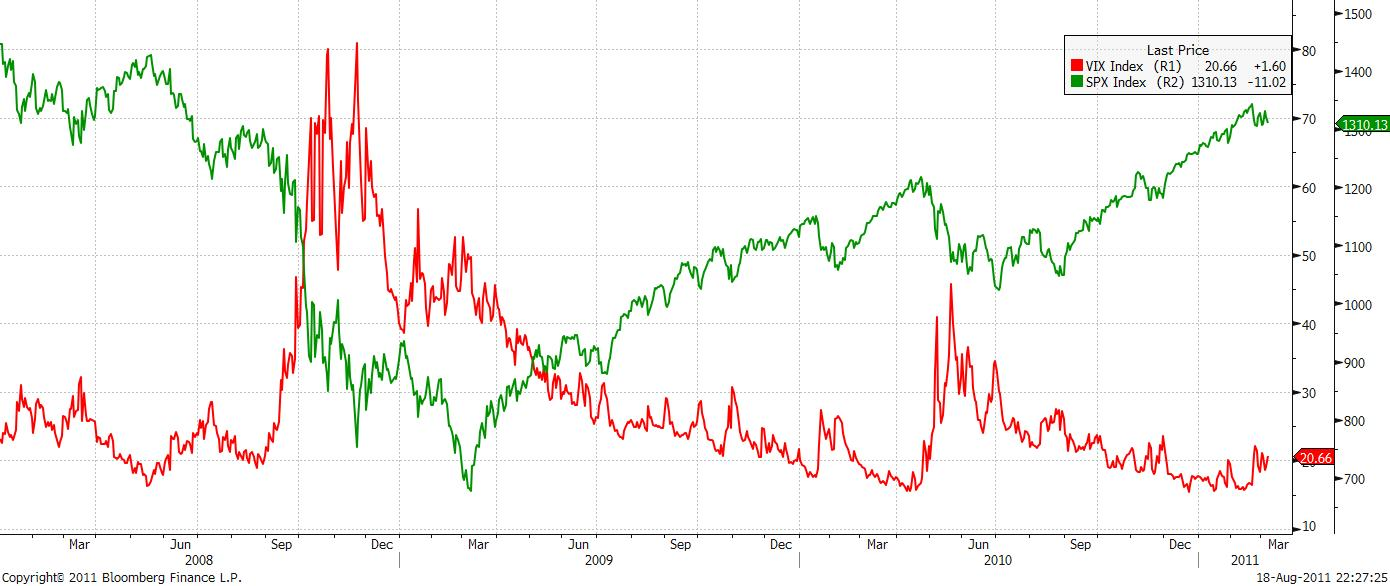
\includegraphics[width=150mm]{vix.jpg}
  \caption{Zmieność w czasie indeksu S\&P}\label{fig:vix}
\end{figure}


gdzie parametr $\sigma$ jest stały. Założenie to jednak okazuję się być zbyt upraszczające dla szerokiej gamy szeregów czasowych. Spojrzmy np. na szereg czasowy  (\ref{fig:vix}) 



\begin{equation}\label{h:ito}
dv(t) = [\delta^2 - 2 \beta v(t)] dt + 2\beta \sqrt{v(t)} dz_2(t),
\end{equation}

The (\ref{h:ito}) equation can be rewritten to the following, square root process

\begin{equation}\label{h:squareroot}
dv(t) = \kappa [\theta - v(t)] dt + \sigma \sqrt{v(t)} d_2 (t),
\end{equation}


\section{Motywacja}
Przedstawiony w poprzednim podrozdziale model Hestona jest bardziej skomplikowany, a niżeli często używony model Blacka-Scholesa, jednak.
Badania empiryczne dowiodły, że logarytmiczne rozkłady stóp zwrotu nie są gausowskie. To znaczy, mają grube ogony oraz charakteryzują się leptokurtozą.

Ostatni kryzys finansowy z lat 2007-2008 pokazuje, ze założenie o stałej zmienności nie moze zostać uznane za prawdziwe w większości instrumentów finansowych jakie są obecnie handlowane na rynku. Dlatego też 


\section{Dyskretyzacja Eulera}
 Jak wynika ze wzorów  

  
\section{Generowanie skorelowanych szeregów czasowych}
W tej sekcji zajmiemy się generowanie skorelowanych szeregów czasowych o zadanym stopniu korelacji $\rho$.
Jednym z ważniejszych zagadnienień związanych z użyciem modelu Hestona jest odpowiednie generowanie skorelowanych szeregów czasowych. Algorytm , przedstawiony w zaloaczniku do pracy opisuje, jak majac dwa kontenery z wartościami z rozkładu jednostajnego możemy wygenerować nowy wektor o zadanej korelacji $\rho$ w stosunku do pierwszego kontenera z danymi. 

Poniższy wykres przedstawia wygenerowane przekladowe szeregi czasowe z zadanym poziomem korelacji na poziomie $\rho = 0.2$:

\begin{figure}
  \centering
  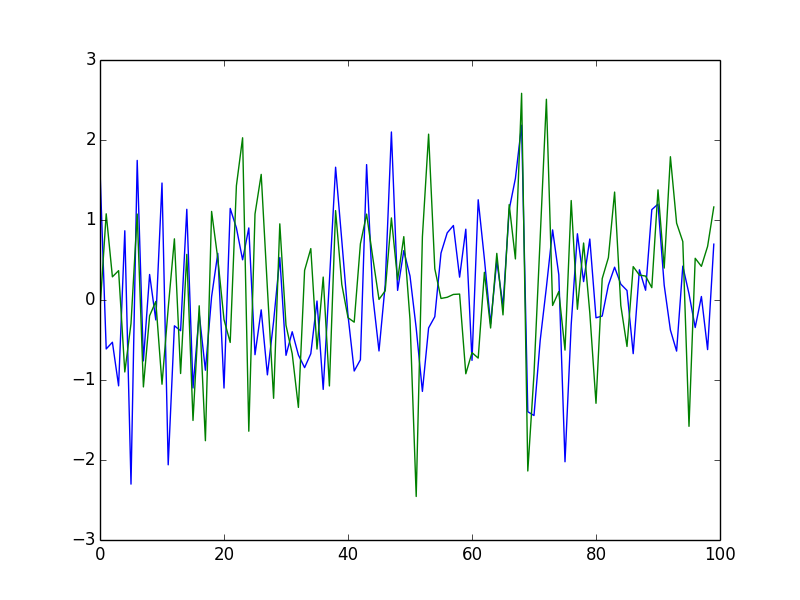
\includegraphics[width=150mm]{corr.png}
  \caption{Zmieność w czasie indeksu S\&P}\label{fig:vix}
\end{figure}

Majac w ten sposób wyznaczone szeregi czasowe o zadanym poziomie korelacji teraz przychodzi czas na generowanie szeregu czasowego opisujacym zmienność oraz samą cenę instrumentu finansowego. 
Przypomnijmy, że zgdonie z modelem Hestona wzory te prezentują się następujuąco:

Mając funkcje generujacą skorelowane szergi czasowe mozna zdefiniowac funkcje, ktorej wynikiem bedzie cena instrumentu bazowego w danej chwili. Jej definicja będzie zgodna z następujacym zbiorem formul: \cite{OptimalInvestment2010}

\begin{equation}
dS_t =  \mu S_t  dt + \sqrt{V_t}S_t dW_t^1
\end{equation}

\begin{equation}
dV_t =  \kappa (\theta - V_t)  dt + \sqrt{V_t} dW_t^2
\end{equation}

\begin{equation}
dW_t^1 dW_t^2  = \rho dt
\end{equation}


%===========================================================================
%                       Model Hestona na przykładznie
%===========================================================================
\chapter{Wycena opcji na indeks S\&P}\label{r:sp}
Lorem ipsum
 


%===========================================================================
%                             Zakończenie
%===========================================================================
 \chapter*{Zakończenie}\label{r:ending}
Lorem ipsum



\appendix

\chapter{Basic concepts and definitions}

\begin{verbatim}
[[foo]{,}[[a3,(([(,),{[[]]}]),
  [1; [{,13},[[[11],11],231]]].
  [13;[!xz]].
  [42;[{,x},[[2],{'a'},14]]].
  [br;[XQ*10]].
 ), 2q, for, [1,]2, [..].[7]{x}],[(((,[[1{{123,},},;.112]],
        else 42;
   . 'b'.. '9', [[13141],{13414}], 11),
 [1; [[134,sigma],22]].
 [2; [[rho,-],11]].
 )[14].
 ), {1234}],]. [map [cc], 1, 22]. [rho x 1]. {22; [22]},
       dd.
 [11; sigma].
        ss.4.c.q.42.b.ll.ls.chmod.aux.rm.foo;
 [112.34; rho];
        001110101010101010101010101010101111101001@
 [22%f4].
 cq. rep. else 7;
 ]. hlt
\end{verbatim}
 
 


\begin{center}
  \begin{tabular}{rrr}
    $\alpha$ & $\beta$ & $\gamma_7$ \\
    901384 & 13784 & 1341\\
    68746546 & 13498& 09165\\
    918324719& 1789 & 1310 \\
    9089 & 91032874& 1873 \\
    1 & 9187 & 19032874193 \\
    90143 & 01938 & 0193284 \\
    309132 & $-1349$ & $-149089088$ \\
    0202122 & 1234132 & 918324098 \\
    11234 & $-109234$ & 1934 \\
  \end{tabular}
\end{center}

%\chapter{Exemplary results}

\begin{center}
  \begin{tabular}{lrrrr}
    & Coefficients \\
    & haha & $\rho$ & $\sigma$ & $\sigma$-$\rho$\\
    $\gamma_{0}$ & 1,331 & 2,01 & 13,42 & 0,01 \\
    $\gamma_{1}$ & 1,331 & 113,01 & 13,42 & 0,01 \\
    $\gamma_{2}$ & 1,332 & 0,01 & 13,42 & 0,01 \\
    $\gamma_{3}$ & 1,331 & 51,01 & 13,42 & 0,01 \\
    $\gamma_{4}$ & 1,332 & 3165,01 & 13,42 & 0,01 \\
    $\gamma_{5}$ & 1,331 & 1,01 & 13,42 & 0,01 \\
    $\gamma_{6}$ & 1,330 & 0,01 & 13,42 & 0,01 \\
    $\gamma_{7}$ & 1,331 & 16435,01 & 13,42 & 0,01 \\
    $\gamma_{8}$ & 1,332 & 865336,01 & 13,42 & 0,01 \\
    $\gamma_{9}$ & 1,331 & 34,01 & 13,42 & 0,01 \\
    $\gamma_{10}$ & 1,332 & 7891432,01 & 13,42 & 0,01 \\
    $\gamma_{11}$ & 1,331 & 8913,01 & 13,42 & 0,01 \\
    $\gamma_{12}$ & 1,331 & 13,01 & 13,42 & 0,01 \\
    $\gamma_{13}$ & 1,334 & 789,01 & 13,42 & 0,01 \\
    $\gamma_{14}$ & 1,331 & 4897453,01 & 13,42 & 0,01 \\
    $\gamma_{15}$ & 1,329 & 783591,01 & 13,42 & 0,01 \\
  \end{tabular}
\end{center}

\listoffigures
\addcontentsline{toc}{chapter}{List of figures} \markboth{Figures}{}
\listoftables
\addcontentsline{toc}{chapter}{List of tables} \markboth{Tables}{}



\chapter*{Bibliography}
\addcontentsline{toc}{chapter}{Bibliography} \markboth{Bibliography}{}

\begin{quote}
"Widziałem dalej dzięki temu, że stałem na barkach gigantów".\\
%(If I have seen farther than others, it is because I was standing on the shoulders of giants).

\raggedleft\slshape Isaac Newton
\end{quote}
 

\printbibliography

\printindex
\end{document}


%%% Local Variables:
%%% mode: latex
%%% TeX-master: t
%%% coding: latin-2
%%% End: